\documentclass[]{article}
%\usepackage[scaled=.92]{helvet}
\usepackage{times}
\usepackage{graphicx}
\usepackage[section] {placeins}
\usepackage{float}
%%* Dica: use esse pacote pra aceitar caracteres acentuados, Ç etc sem sofrimento
%%* obs: válido se estiverem escrevendo com codificação Windows, caso contrário
%%* pode ser necessário trocar ansinew por utf8 ou algo assim.
\usepackage[ansinew]{inputenc}

%% use this for zero \parindent and non-zero \parskip, intelligently.
\usepackage{parskip}

%% the 'caption' package provides a nicer-looking replacement
\usepackage[labelfont=bf,textfont=it]{caption}

\usepackage{url}
\usepackage{listings}
\usepackage{color}
\usepackage{graphicx}

% %\lstset{language=C++,breaklines=true,morekeywords={float3,float4},keywordstyle=\color[rgb]{0,0,1},        commentstyle=\color[rgb]{0.133,0.545,0.133} }


%opening
\title{}
\author{Bruno Duarte Correa}

\begin{document}

\maketitle

\begin{abstract}
Recognition of objects in a scene for later use in augmented reality depends on several variables, causing the need 
to use several specific techniques for each scenario, and therefore a border
analysis to the best choice of the registration algorithm according to
application in question, of great value to academia.
This thesis aims to examine, categorize and draw boundaries of the known techniques having as use case maintenance of 
aircraft made in closed center, using the techniques BRISK,FAST,FREAK,GFTT,MSER,
ORB,STAR,SURF,SIFT in an applied analysis with images of the Embraer ERJ-190 to recognition of objects and future usage in maintenance. Comparing all of the techniques, using cadency and recognition precision, it is possible to chose GFTT and ORB as the most appropriate ones because its results to the variation of
rotation, scale, brightness and blur fulfils the constraints needed



\end{abstract}



\section{Introduction}
Based primarily on the parameters cited on the spec phase leading to decrease the maintenance cost and increase the profit.


The main modification guided by market forecasting the possibility of a more passenger reality in the world by increasing to 60 seats adding a new fuselage section.


To reduce the airplane weight all the illumination were replaced to LED instead of regular lamps what indirectly decreases the maintenance costs. The replacement of the seat was guided to decrease the pitch in the cabin and enable the increase of seats without increasing the fuselage so much, choosing a 29" pitch seat.


An operator galley usage analysis guided the decision of decrease its number but not its necessary volume.
All decisions made were also mockup driven to validate comfort and ergonomics.




\section{Concepts}
\subsection{Camera}
\subsection{Camera Calibration}
\subsection{SLAM}
\subsection{Structure from Motion (SfM)}
\subsection{Edge Recognition}

\section{Method}
The recognition of an object in a scene with precision can be a trick problem to be solved, and to increase the experience with some virtual artifacts calls for a high level of localization accuracy.

This paper presents an approach based a pre-known 3d representation of the scene.

The real time reconstruction of the scene are fundamental to reduce the cumulative error added to the recognition added after each frame because of interest point recognition hardness caused by light variation, textures and other issues studied in this essay.
As proposed in \cite{ISMAR2012}

\begin{figure}[ht!]
\centering
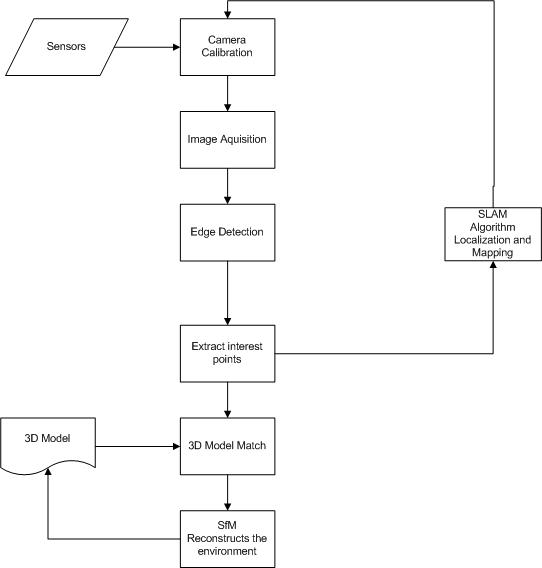
\includegraphics[width=90mm]{images/algorithm.jpg}
\caption{Algorithm Diagram}
\label{algorithm}
\end{figure}


O caminho feliz é ditado por aquisição de imagem, reconhecimento de bordas, reconhecimento de pontos de interesse, model match reconhecimento de 



\subsection{AR Common Flaws}

Jitter
Occlusion

\subsection{Camera Calibration}

\subsubsection{Error Reduction Approach}

Todo frame com a movimentação da camera ou do objeto o rastreamento descasa um pouco, prejudicando a precisão.
Dois métodos são utilizados para reduzir o erro de rastreamento
SLAM utilizado para conferir uma calibracao boa recuperando informacoes de movimento e tentando inferir a posicao da camera


Tenho que ver como vou medir o erro a cada frame, se vai ser um minimo quadrados de pontos importantes com o modelo ou algo mais robusto


\subsection{Image Acquisition}

Etapa simples, tenho que definir qual a latencia de aquisicao de imagens que terei uma quantidade de informacoes suficiente, aqui cabe colocar uma variável para calcular o erro final

\subsection{Edge Detection}

Obter as bordas para depois conseguir retirar os pontos de interesse, aqui cabem filtros ou reconhecedores de padrao.

Também é outra fonte de erro adicionada ao final do modelo.

\cite{Drummond99real-timetracking}


\subsection{Extract Interest Points}

Dependendo do reconhecedor de padrão conseguirei retirar um tipo de ponto de interesse diferente.

Aqui terei uma miriade de reconhecedores que podem adicionar erros ou incertezas ao modelo

\subsection{Model Match}


Eu acho que é a parte que vai mais dar trabalho porque eu vou ter que provavelmente estimar pose para definir projecoes diferentes

\subsubsection{Choosing the apropriate approach to 3d track}



\subsubsection{Real Time Model Reconstruction}

Quando reconhecermos e 


\subsubsection{SLAM}




\section{Boundaries}
% %Nessa seção serão descritos as fronteiras que desejam ser estudadas bem como porque elas são relevantes


\section{Study Case}
\input{parts/results}

\section{Conclusion}
%% ---------- Conclusion ---------- %%

The study main objective was to verify the technical and economical viability of the 145 modification on structures point of view, as mentioned before, most of the studies were a demand from aeronautics group due to the high integration between those two.

In the end, the analysis has shown the only small changes were necessary to guarantee the aircraft good safety margin and fulfill the regulations. The costs of those changes were smaller than initially thought as well as the necessary reinforcements.


\bibliography{bibliography}
\bibliographystyle{ieeetr}

\end{document}
